\documentclass[12pt]{unlsilabsop}
\title{Visual inspection of assembled modules}
\date{August 6, 2015}
\author{Frank Meier Aeschbacher}
\approved{Frank Meier Aeschbacher}
\sopid{205}
\sopversion{v1}
\sopabstract{Describes the procedures for visual inspection of final modules. This consists mainly of an inspection by eye and using a microscope. Any deviations from normal appearance will be documented.}
\begin{document}

\maketitle

%------------------------------------------------------------------
\section{Scope}
This is a regular test in the manufacturing process of pixel modules at UNL.

%------------------------------------------------------------------
\section{Purpose}
The visual inspection of final modules is a critical step in manufacturing modules. This test is a critical control point to make sure the material we send out meets expectations and to ensure the quality.

%------------------------------------------------------------------
%>\section{Definitions}

%------------------------------------------------------------------
%\section{Responsibilities}

%------------------------------------------------------------------
\section{Equipment}

\begin{itemize}
\item \textbf{Probe station} Jmicro JR-2745, to hold the setup
\item \textbf{Microscope with camera and LED ring illumination} Microscope at probe station, with camera connected to the computer
\item \textbf{Gooseneck LED lamps} mounted on microscope stand
\item \textbf{Computer} Requires ToupeViewX installed (software to grab images from microscope camera) and ImageMagick
\item \textbf{Binder clips} 15\,mm wide, inside insulated with Kapton tape
\end{itemize}

%------------------------------------------------------------------
\section{Procedure}

\begin{enumerate}
    \item Handle modules only with proper protection: ESD wristband, gloves, face mask.
    \item A protective Kapton-insulated binder clip has to be attached to the dangling end of the flex cable whenever modules are stored or handled when no ESD protection can be worn (e.g.~when transferring modules on closed carriers between cleanroom and test stand).
    \item Place the module on the probe station. Turn on the vacuum.
    \item Remove the module cover, in case it is attached. For this, open the four screws by hand, set them aside and lift of the cover.
    \item Check if the flex cable is properly inserted. If yes, keep it. If no flex cable is present insert one. This needs to be done in the clean room.
    \item Take note of identifying information printed on the HDI: work order, manufacturing week and year, panel and position numbers. Use this to retrieve the module from the database.

    \begin{center}
        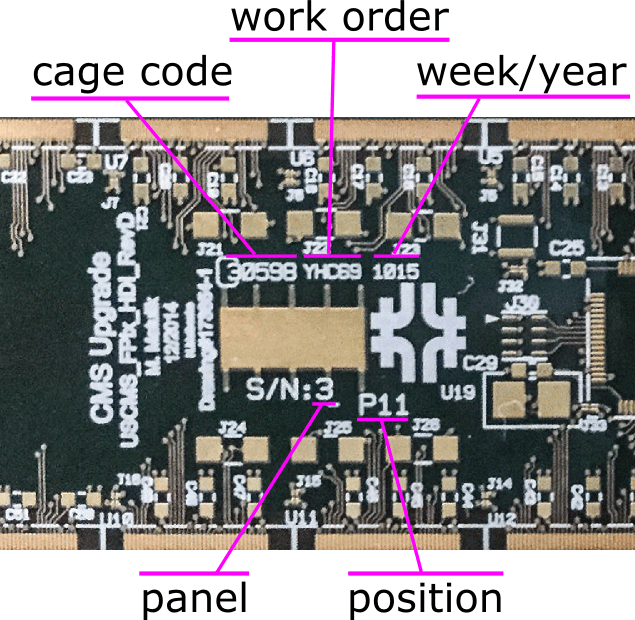
\includegraphics[width=5cm]{img/HDIRevD_id.png}
    \end{center}

    \item Start up camera software on computer
    \item Starting on the top left corner, zoom in with microscope until the field of vision from left to right is approximately the width of one ROC (=group of 35 bond pads). The red circled areas shown in the image are areas of special interest where wire bonds need to be checked in the next few steps.

    \begin{center}
        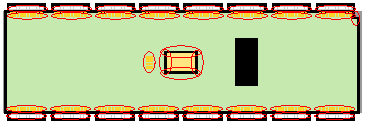
\includegraphics[width=9cm]{img/ModuleSchematicInpsection.pdf}
    \end{center}

    \item Inspect all wirebonds. They need to be present, intact and of good shape. The encapsulant needs to be present and cover the full bond pads, but not the entire bond. The images below show a good and a bad example, in the latter case the pads are not fully covered on the HDI side. The encapsulant is shown as a transparent blue-ish area.

    \begin{center}
        \begin{tabular}{cc}
        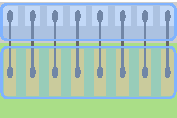
\includegraphics[width=3cm]{img/PottingGood.pdf} & 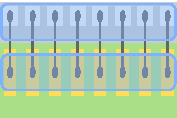
\includegraphics[width=3cm]{img/PottingBad.pdf} \\
        Good & Bad \\
        \end{tabular}
    \end{center}

    \item Move the table using the knob. Scan both long edges of the module and check for any obvious damage or dirt. Check the bonds and encapsulation.
    \item Move to the center where the TBM chip is mounted. Check the bonds and encapsulation.
    \item Move to the neighboring wirebonds that set the module address. Check the bonds and encapsulation.
    \item Document any findings. Any damage visibile or unusual feature needs to be documented using a picture. Adjust the exposure in a way to capture bright and dark areas at the same time. If needed, adjust lighting conditions. The controller for the LED ring allows to adjust the brightness and switch quadrants on and off. Label files with a clear reference to the module and the position this image shows.
\end{enumerate}
\textbf{Note:} The image capturing software only allows to store bitmap files (\texttt{*.bmp}), which are too large to be stored in the database or the elog. To convert files, use ImageMagick from the command line as follows:

\medskip

\texttt{\$> convert -resize 1024x768 filename.\{bmp,jpg\}} 
\medskip

where \texttt{filename.bmp} is the name of the file given when the image got saved in the camera capture software.

%------------------------------------------------------------------
\section{Documentation}
This inspection is part of the final testing and usually before the electrical tests have been carried out. Therefore, no status update in the database needed. But to document any finding, go to ``MAIN MENU''$\rightarrow$``Part List'' and select your module. Upload any pictures as needed and add comments as needed.

No need to make an entry in the Elog if nothing special happened.

\end{document}

